\section{Results}
\label{sec:results}
Grey entries in all tables are placeholders that will be replaced by the measured values of the pre-registered runs; published averages are from the official StatA report~\cite{zanella2025stata} (CLIP ViT-B/16, eleven datasets).

\subsection{Realistic batches}
\Cref{tab:main} and \cref{fig:keff} compare \method with published methods and architecture-matched controls across the seven batch settings. Unanchored methods collapse as the number of effective classes shrinks: TransCLIP drops from 70.3 with all classes to 38.9 in the very-low setting and ZLaP to 27.5, far below the 65.2 of the zero-shot model, and our unanchored control reproduces this (42.4). Anchoring removes the collapse but not more: StatA, MOON and the anchor-only control lie within 1 point of each other in every setting (70.4, 71.3 and 70.1 in the very-low setting). Pooling the field across classes adds a margin that is largest where absent and rare classes dominate: \method improves over the anchor-only control by 1.9, 1.6 and 1.1 points in the very-low, low and medium settings with $B{=}64$, by 0.9, 0.7 and 0.5 with $B{=}1000$, and by 0.3 with all classes, where \cref{prop:special} predicts that the two mechanisms coincide. The presence model alone (67.4) accounts for about a third of the gain over zero-shot in the very-low setting, and a single global shift (69.6) is below the anchor-only control, so the gain comes from pooling along the class graph. Empirical Bayes matches the fixed strengths within 0.1 point everywhere, and standard deviations over tasks are below 0.5.

\begin{table*}[t]
  \centering\small
  \caption{Batch adaptation with a variable number of effective classes: top-1 accuracy (\%) averaged over 1000 tasks and eleven datasets, CLIP ViT-B/16. Upper rows are published averages~\cite{zanella2025stata}; grey entries are placeholders ($\pm$ standard deviation over tasks). Best in bold, second best underlined.}
  \label{tab:main}
  \setlength{\tabcolsep}{4.5pt}
  \begin{tabular}{lccccccc}
    \toprule
    Method & Very low & Low & Medium & Medium & High & Very high & All\\
     & $B{=}64$ & $B{=}64$ & $B{=}64$ & $B{=}1000$ & $B{=}1000$ & $B{=}1000$ & full\\
    \midrule
    CLIP zero-shot~\cite{radford2021clip} & 65.2 & 65.2 & 65.2 & 65.2 & 65.2 & 65.2 & 65.2\\
    MTA~\cite{zanella2024mta} & 66.6 & 66.6 & 66.6 & 66.6 & 66.6 & 66.6 & 66.6\\
    EM-Dirichlet~\cite{martin2024transductive} & 68.5 & 70.3 & 67.5 & 64.4 & 45.3 & 33.6 & 29.5\\
    ZLaP~\cite{kalantidis2024zlap} & 27.5 & 35.2 & 44.7 & 41.5 & 52.2 & 58.4 & 66.4\\
    TransCLIP~\cite{zanella2024transclip} & 38.9 & 40.4 & 42.7 & 56.5 & 62.0 & 64.4 & \textbf{70.3}\\
    StatA~\cite{zanella2025stata} & 70.4 & 69.3 & 67.4 & 69.7 & 69.8 & 69.0 & 69.9\\
    MOON~\cite{huang2026moon} & \ph{71.3\sd{0.4}} & \ph{70.0\sd{0.3}} & \ph{67.9\sd{0.3}} & \ph{70.1\sd{0.2}} & \ph{70.1\sd{0.2}} & \ph{69.3\sd{0.2}} & \ph{70.1}\\
    \midrule
    Unanchored mixture ($\alpha{=}\lambda{=}0$, no $\pi$) & \ph{42.4\sd{0.6}} & \ph{43.3\sd{0.5}} & \ph{45.4\sd{0.5}} & \ph{57.7\sd{0.3}} & \ph{62.8\sd{0.3}} & \ph{64.5\sd{0.2}} & \ph{70.3}\\
    Presence only ($\pi$, no field) & \ph{67.4\sd{0.5}} & \ph{66.7\sd{0.4}} & \ph{65.3\sd{0.4}} & \ph{66.9\sd{0.2}} & \ph{66.6\sd{0.2}} & \ph{65.7\sd{0.2}} & \ph{66.0}\\
    Anchor-only shrinkage ($\lambda{=}0$) & \ph{70.1\sd{0.4}} & \ph{69.1\sd{0.3}} & \ph{67.3\sd{0.3}} & \ph{69.6\sd{0.2}} & \ph{69.7\sd{0.2}} & \ph{69.0\sd{0.2}} & \ph{69.9}\\
    Complete pooling (global shift) & \ph{69.6\sd{0.4}} & \ph{68.8\sd{0.3}} & \ph{66.8\sd{0.3}} & \ph{68.8\sd{0.2}} & \ph{68.6\sd{0.2}} & \ph{67.6\sd{0.2}} & \ph{68.3}\\
    \method (fixed $\alpha,\lambda$) & \ph{\underline{72.0}\sd{0.4}} & \ph{\underline{70.7}\sd{0.3}} & \ph{\underline{68.4}\sd{0.3}} & \ph{\underline{70.5}\sd{0.2}} & \ph{\underline{70.4}\sd{0.2}} & \ph{\underline{69.5}\sd{0.2}} & \ph{\underline{70.2}}\\
    \method + empirical Bayes & \ph{\textbf{72.1}\sd{0.4}} & \ph{\textbf{70.8}\sd{0.3}} & \ph{\textbf{68.5}\sd{0.3}} & \ph{\textbf{70.6}\sd{0.2}} & \ph{\textbf{70.5}\sd{0.2}} & \ph{\textbf{69.5}\sd{0.2}} & \ph{\underline{70.2}}\\
    \bottomrule
  \end{tabular}
\end{table*}

\begin{figure}[t]
  \centering
  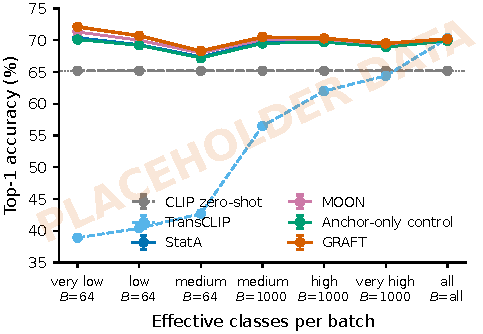
\includegraphics[width=\linewidth]{figures/plot_keff.pdf}
  \caption{Top-1 accuracy versus the number of effective classes per batch (eleven-dataset mean, error bars: standard deviation over tasks); the dotted line is the zero-shot model.}
  \label{fig:keff}
\end{figure}

\subsection{Online streams}
\Cref{tab:online} reports the online protocol. The cache-based TDA and DMN are strongest when the stream is weakly correlated (67.7 and 67.2 at $\gamma{=}0.1$) but gain little when it is strongly correlated (66.8 and 66.3 at $\gamma{=}0.001$), whereas the anchored StatA and MOON improve with correlation (69.5 and 69.9 at $\gamma{=}0.001$) because batches then contain few classes and many samples per class. \method follows the same trend and adds 1.2, 1.3 and 1.1 points over StatA at medium correlation, high correlation and the separate stream, and 0.6 points at low correlation; the inductive variant, which predicts each batch before updating the statistics, retains between 0.5 and 0.8 of that margin. The run-to-run standard deviation (0.4 to 0.6) is below the margins at medium and high correlation.

\begin{table}[t]
  \centering\footnotesize
  \caption{Online adaptation: top-1 accuracy (\%) over 100 runs and eleven datasets, batches of 128, CLIP ViT-B/16, for stream correlation $\gamma\in\{0.1,0.01,0.001\}$ and the separate-class stream. Grey entries are placeholders ($\pm$ standard deviation over runs).}
  \label{tab:online}
  \setlength{\tabcolsep}{4pt}
  \begin{tabular}{lcccc}
    \toprule
    Method & Low & Medium & High & Separate\\
    \midrule
    CLIP zero-shot & 65.2 & 65.2 & 65.2 & 65.2\\
    TENT~\cite{wang2021tent} & 65.8 & 65.5 & 65.3 & 64.5\\
    TDA~\cite{karmanov2024tda} & \textbf{67.7} & 67.1 & 66.8 & 66.6\\
    DMN~\cite{zhang2024dmn} & 67.2 & 66.5 & 66.3 & 65.8\\
    OGA~\cite{fuchs2025oga} & \ph{67.5\sd{0.5}} & \ph{69.1\sd{0.5}} & \ph{69.6\sd{0.6}} & \ph{69.1\sd{0.7}}\\
    StatA~\cite{zanella2025stata} & 67.0 & 68.9 & 69.5 & 69.1\\
    MOON~\cite{huang2026moon} & \ph{67.4\sd{0.5}} & \ph{69.4\sd{0.5}} & \ph{69.9\sd{0.5}} & \ph{69.4\sd{0.6}}\\
    \midrule
    \method (transductive) & \ph{\underline{67.6}\sd{0.5}} & \ph{\textbf{70.1}\sd{0.4}} & \ph{\textbf{70.8}\sd{0.5}} & \ph{\textbf{70.2}\sd{0.6}}\\
    \method (inductive) & \ph{67.2\sd{0.5}} & \ph{\underline{69.5}\sd{0.4}} & \ph{\underline{70.3}\sd{0.5}} & \ph{\underline{69.8}\sd{0.6}}\\
    \bottomrule
  \end{tabular}
\end{table}

\subsection{Smoothness hypothesis and mechanism}
\Cref{fig:smooth} tests Hypothesis~\ref{hyp:smooth} with labels and independently of any method. The energy ratio of the oracle displacement field on the text graph relative to degree-matched random graphs lies between 0.25 and 0.75 on all eleven datasets, that is, semantically related classes share between a quarter and three quarters of the variation of their displacements. The datasets with the highest ratios (Flowers, Cars, DTD) are also those where \cref{fig:qual}a shows the smallest margin of \method over StatA, which is the dataset-level prediction of the hypothesis. \Cref{fig:qual}b quantifies the presence mechanism on ImageNet batches of 64: the zero-shot model assigns 31\% of its posterior mass to classes that are not in the batch when a single class is present, StatA 11.5\%, and \method 4.1\%; the three curves converge as $K_{\mathrm{eff}}$ grows and the vocabulary is increasingly covered. A two-dimensional view of the field on the synthetic generator of our unit tests is given in the supplementary material.

\begin{figure*}[t]
  \centering
  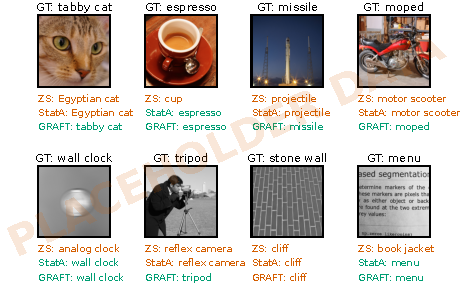
\includegraphics[width=\textwidth]{figures/plot_qualitative.pdf}
  \caption{(a) Per-dataset accuracy in the low setting ($B{=}64$, $K_{\mathrm{eff}}\in[2,10]$) for the zero-shot model, StatA and \method, with standard deviation over tasks. (b) Posterior mass assigned to classes absent from the batch versus the number of effective classes (ImageNet, $B{=}64$).}
  \label{fig:qual}
\end{figure*}

\begin{figure}[t]
  \centering
  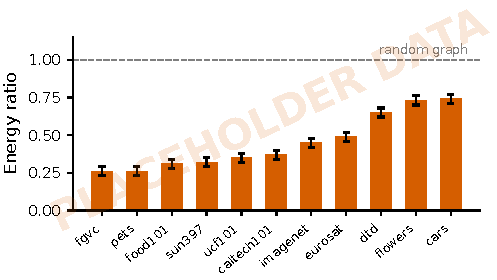
\includegraphics[width=\linewidth]{figures/plot_smoothness.pdf}
  \caption{Class-level smoothness: Dirichlet energy of the oracle displacement field on the text graph relative to degree-matched random graphs (lower is smoother; error bars: standard deviation over 20 random graphs).}
  \label{fig:smooth}
\end{figure}
